\documentclass[aspectratio=169, table, 12pt]{beamer}

\usepackage{colortbl}
\usepackage{xcolor}
\usepackage{listings}
\usepackage{tabularx}
\usepackage{tikz}
\usetikzlibrary{arrows.meta, positioning, calc, fit, shapes.geometric}

\makeatletter
\def\input@path{{../theme/}}
\makeatother
\graphicspath{{../theme/}{../../figures/}}
\usetheme{Pradita}

\definecolor{praditagreen}{RGB}{37, 113, 71}

% Tema membuat garis tabel berwarna putih. Dikembalikan agar tabel terbaca.
\arrayrulecolor{black}
\setlength{\arrayrulewidth}{0.5pt}

% Kolom X rata kiri, dipakai pada tabel dengan kolom X yang sempit, agar
% spasi antarkata tidak meregang.
\newcolumntype{Y}{>{\raggedright\arraybackslash}X}

\lstdefinelanguage{bash}{
  keywords={},
  basicstyle=\ttfamily\scriptsize,
  ndkeywords={cd, coverage, curl, diff, docker, echo, npm, npx, python,
              python3, pytest, source},
  ndkeywordstyle=\color{purple}\bfseries,
  sensitive=true,
  commentstyle=\color{gray},
  numbers=none,
  breaklines=true,
  frame=lines,
  backgroundcolor=\color{lightgray!10},
  tabsize=2,
  comment=[l]{\#},
  showstringspaces=false
}

\lstdefinelanguage{TypeScript}{
  keywords={const, let, function, return, async, await, try, catch, throw,
            new, if, interface, void, export, import, from, type},
  ndkeywords={Promise, number, string, boolean, test, expect, Page, await},
  basicstyle=\ttfamily\scriptsize,
  keywordstyle=\color{blue}\bfseries,
  ndkeywordstyle=\color{purple}\bfseries,
  sensitive=true,
  commentstyle=\color{gray}\itshape,
  stringstyle=\color{red},
  numbers=none,
  breaklines=true,
  frame=lines,
  backgroundcolor=\color{lightgray!10},
  tabsize=2,
  comment=[l]{//},
  morestring=[b]",
  showstringspaces=false
}

% Gaya Python disamakan dengan naskah bab, tanpa nomor baris.
\lstdefinestyle{PythonStyle}{
  language=Python,
  basicstyle=\ttfamily\scriptsize,
  morekeywords={with, as, yield, async, await, match, case},
  keywordstyle=\color{blue}\bfseries,
  emph={pytest, psycopg, Mock, given, strategies},
  emphstyle=\color{purple}\bfseries,
  commentstyle=\color{gray}\itshape,
  stringstyle=\color{red},
  numbers=none,
  breaklines=true,
  frame=lines,
  backgroundcolor=\color{lightgray!10},
  tabsize=2,
  showstringspaces=false
}

% File mutu dan kontrak ditampilkan apa adanya, sehingga butuh gaya JSON.
\lstdefinelanguage{json}{
  basicstyle=\ttfamily\scriptsize,
  stringstyle=\color{red},
  commentstyle=\color{gray},
  numbers=none,
  breaklines=true,
  frame=lines,
  backgroundcolor=\color{lightgray!10},
  tabsize=2,
  showstringspaces=false,
  morestring=[b]"
}

\title{\Huge Identity, Authentication,\\ \vspace{10pt} dan Authorization}
\subtitle{IF140303 - Pengembangan Aplikasi Web}
\author{\textbf{Alfa Yohannis}}

\begin{document}

\frame{\titlepage}

\begin{frame}[fragile]
  \frametitle{Isi Pertemuan}
  \vspace{14pt}
  \begin{columns}[t]
    \column{0.5\textwidth}
    {\small\tableofcontents[sections={1-7}]}

    \column{0.5\textwidth}
    {\small\tableofcontents[sections={8-14}]}
  \end{columns}
\end{frame}

\begin{frame}{\hfill}
  \centering
  \Huge{\textbf{Siapa yang meminta,\\dan apa yang boleh dilakukannya?}}
\end{frame}

\section{Tujuan dan Kerangka Bahasan}

\begin{frame}{\hfill}
  \centering
  \Huge{\textbf{Tujuan dan Kerangka Bahasan}}
\end{frame}

\begin{frame}{{\Large Tujuan Pembelajaran}}
  \vspace{10pt}
  \begin{itemize}
    \item Membedakan sesi yang disimpan server dari token bertanda tangan,
          lalu menyebut akibatnya pada pencabutan.
    \item Merancang pasangan \textit{access token} dan \textit{refresh
          token} beserta rotasinya, lalu membuktikan pemakaian ulang penanda
          lama tertangkap.
    \item Menegakkan hak akses dengan RBAC dan ABAC sekaligus, lalu
          mengukurnya sebagai matriks pengguna lawan alamat.
  \end{itemize}
\end{frame}

\begin{frame}{{\Large Dua Pertanyaan yang Sering Disatukan}}
  \vspace{12pt}
  \begin{itemize}
    \item \textbf{\textit{Authentication}} menjawab siapa, dan jawabannya
          satu kali di awal.
    \item \textbf{\textit{Authorization}} menjawab boleh atau tidak, dan
          jawabannya diulang pada tiap permintaan.
  \end{itemize}
  \vspace{10pt}
  {\small Kesalahan paling mahal biasanya di pertanyaan kedua: aplikasi
  mengenali penggunanya dengan benar, lalu lupa memeriksa apa yang boleh
  dilihatnya.}
\end{frame}

\section{Cookie dan Session}

\begin{frame}{\hfill}
  \centering
  \Huge{\textbf{Cookie dan Session}}
\end{frame}

\begin{frame}[fragile]{{\Large Sesi Dicabut Seketika}}
  \vspace{2pt}
\begin{lstlisting}[language=bash]
curl -s -X POST "http://127.0.0.1:8070/masuk?cara=sesi&nama=budi&sandi=budi123" -D -
curl -s -H "Cookie: sesi=..." http://127.0.0.1:8070/api/pesanan
curl -s -X POST -H "Cookie: sesi=..." http://127.0.0.1:8070/keluar
curl -s -H "Cookie: sesi=..." http://127.0.0.1:8070/api/pesanan

# Keluarannya:
# Set-Cookie: sesi=4b2f8d7e...; HttpOnly; SameSite=Lax; Path=/
# {"tenant": "kampus-a", "jumlah": 2, "item": [...]}
# {"dicabut": true}
# {"pesan": "sesi tidak dikenal atau sudah dicabut"}
\end{lstlisting}
  \vspace{2pt}
  {\small Analoginya nomor antrean: kertasnya tidak memuat apa-apa selain
  nomor, dan seluruh keterangan ada di buku petugas.}
\end{frame}

\section{JSON Web Token}

\begin{frame}{\hfill}
  \centering
  \Huge{\textbf{JSON Web Token}}
\end{frame}

\begin{frame}{{\Large Sesi lawan Token, Diukur}}
  \vspace{6pt}
  \centering
  {\footnotesize
  \begin{tabularx}{\textwidth}{Yll}
    \hline
    \textbf{Hal} & \textbf{Sesi} & \textbf{Token} \\
    \hline
    Yang dibawa klien & penanda 32 huruf & token 169 byte \\
    \hline
    Yang disimpan server & arti tiap penanda & tidak ada \\
    \hline
    Dicabut saat keluar & seketika & menunggu kedaluwarsa \\
    \hline
    Hilang saat proses mati & ya & tidak \\
    \hline
    Isinya terbaca klien & tidak & ya, tetapi tidak dapat diubah \\
    \hline
  \end{tabularx}}

  \vspace{8pt}
  {\small Token yang diubah satu huruf langsung ditolak, tetapi isinya tetap
  terbaca siapa pun yang memegangnya. Karena itu token tidak pernah diisi
  data rahasia.}
\end{frame}

\section{OAuth 2.x dan OpenID Connect}

\begin{frame}{\hfill}
  \centering
  \Huge{\textbf{OAuth 2.x\\dan OpenID Connect}}
\end{frame}

\begin{frame}{{\Large Empat Peran pada OAuth}}
  \vspace{10pt}
  \centering
  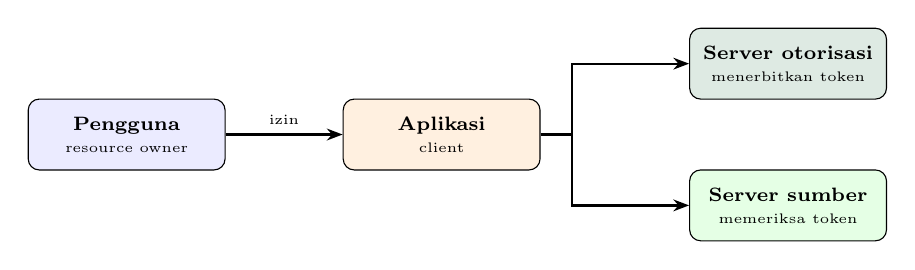
\begin{tikzpicture}[
    font=\scriptsize,
    kotak/.style={draw, rounded corners, minimum height=0.9cm,
                  minimum width=2.5cm, align=center, font=\scriptsize\bfseries},
    panah/.style={-{Stealth[length=2mm]}, thick}
  ]
    \node[kotak, fill=blue!8] (pengguna) at (0,0) {Pengguna\\{\tiny\mdseries resource owner}};
    \node[kotak, fill=orange!12] (klien) at (4.0,0) {Aplikasi\\{\tiny\mdseries client}};
    \node[kotak, fill=praditagreen!15] (otoritas) at (8.4,0.9) {Server otorisasi\\{\tiny\mdseries menerbitkan token}};
    \node[kotak, fill=green!10] (sumber) at (8.4,-0.9) {Server sumber\\{\tiny\mdseries memeriksa token}};

    \draw[panah] (pengguna) -- node[font=\tiny, above] {izin} (klien);
    \draw[panah] (klien.east) -- ++(0.4,0) |- (otoritas.west);
    \draw[panah] (klien.east) -- ++(0.4,0) |- (sumber.west);
  \end{tikzpicture}

  \vspace{10pt}
  {\small OAuth menjawab apa yang boleh diakses, OIDC menjawab siapa yang
  sedang masuk. Memakai \textit{access token} untuk menyimpulkan identitas
  adalah kesalahan yang sering terjadi.}
\end{frame}

\section{Access Token dan Rotasi}

\begin{frame}{\hfill}
  \centering
  \Huge{\textbf{Access Token, Refresh Token,\\dan Rotasinya}}
\end{frame}

\begin{frame}{{\Large Umur Lima Detik, Diukur}}
  \vspace{6pt}
  \centering
  {\footnotesize
  \begin{tabularx}{\textwidth}{Yll}
    \hline
    \textbf{Kapan dipakai} & \textbf{Status} & \textbf{Alasan} \\
    \hline
    Segera sesudah terbit & 200 & sah \\
    \hline
    Sesudah 2 detik & 200 & sah \\
    \hline
    Sesudah 6 detik & 401 & token kedaluwarsa \\
    \hline
    Diubah satu huruf & 401 & tanda tangan tidak cocok \\
    \hline
  \end{tabularx}}

  \vspace{8pt}
  {\small \textit{Access token} ikut terkirim pada tiap permintaan, sehingga
  umurnya pendek. \textit{Refresh token} hanya dikirim ke satu alamat,
  sehingga umurnya boleh panjang.}
\end{frame}

\begin{frame}{{\Large Rotasi Menangkap Pemakaian Ulang}}
  \vspace{6pt}
  \centering
  {\footnotesize
  \begin{tabularx}{\textwidth}{Yll}
    \hline
    \textbf{Langkah} & \textbf{Status} & \textbf{Hasil} \\
    \hline
    Menyegarkan dengan penanda yang sah & 200 & terbit pasangan baru \\
    \hline
    Memakai ulang penanda lama & 401 & dipakai ulang, 2 penanda dicabut \\
    \hline
    Memakai penanda baru sesudah pencabutan & 401 & penanda tidak dikenal \\
    \hline
  \end{tabularx}}

  \vspace{8pt}
  {\small Penanda baru ikut mati karena seluruh keluarganya dicabut. Harga
  itu disengaja: ketika satu penanda terbukti bocor, tidak ada cara
  membedakan pemilik aslinya dari pemegang lainnya.}
\end{frame}

\section{RBAC dan ABAC}

\begin{frame}{\hfill}
  \centering
  \Huge{\textbf{RBAC dan ABAC}}
\end{frame}

\begin{frame}[fragile]{{\Large Tiga Sifat Diperiksa Berurutan}}
  \vspace{2pt}
\begin{lstlisting}[style=PythonStyle]
def boleh_baca_pesanan(identitas, pesanan):
  """Memutuskan satu pesanan boleh dibaca atau tidak, secara ABAC.

  Tiga sifat ikut dibaca: tenant pemohon, tenant pesanan, dan pemiliknya.
  Mengembalikan pasangan (boleh, alasan), sehingga alasan penolakan dapat
  ikut diuji dan ikut dicatat.
  """
  if identitas["tenant"] != pesanan["tenant"]:
    return False, "tenant berbeda"
  if punya_izin(identitas["peran"], "baca_semua_pesanan"):
    return True, "peran boleh membaca seluruh pesanan tenantnya"
  if pesanan["pemilik"] == identitas["sub"]:
    return True, "pemohon adalah pemilik pesanan"
  return False, "bukan pemilik dan perannya tidak mencakup"
\end{lstlisting}
  \vspace{2pt}
  {\small Urutannya penting: pemeriksaan \textit{tenant} paling depan,
  sehingga peran setinggi apa pun tidak menembus batas itu.}
\end{frame}

\section{Multi-Tenancy}

\begin{frame}{\hfill}
  \centering
  \Huge{\textbf{Multi-Tenancy\\dan Isolasi Data}}
\end{frame}

\begin{frame}{{\Large Satu Tabel, Tiga Pelajaran}}
  \vspace{6pt}
  \centering
  {\footnotesize
  \begin{tabularx}{\textwidth}{Yllll}
    \hline
    \textbf{Pengguna} & \textbf{/api/pesanan} & \textbf{/pesanan/1} & \textbf{/pesanan/3} & \textbf{/laporan} \\
    \hline
    ani, admin kampus-a & 200, 2 baris & 200 & 404 & 200 \\
    \hline
    budi, staf kampus-a & 200, 2 baris & 200 & 404 & 403 \\
    \hline
    cita, pembeli kampus-a & 200, 1 baris & 200 & 404 & 403 \\
    \hline
    dedi, staf kampus-b & 200, 1 baris & 404 & 200 & 403 \\
    \hline
  \end{tabularx}}

  \vspace{6pt}
  {\footnotesize Kolom terakhir murni RBAC. Kolom pertama murni ABAC: cita
  hanya melihat pesanan miliknya. Dua kolom tengah memuat isolasi
  \textit{tenant}.}
\end{frame}

\begin{frame}{{\Large Mengapa 404 dan Bukan 403}}
  \vspace{14pt}
  \begin{itemize}
    \item Jawaban 403 berarti "ada, tetapi Anda tidak boleh", dan jawaban itu
          sendiri sudah membocorkan keberadaan datanya.
    \item Permintaan lintas \textit{tenant} karena itu dijawab 404.
    \item Penolakan di dalam satu \textit{tenant} tetap 403, karena di sana
          keberadaan pesanan memang bukan rahasia.
  \end{itemize}
  \vspace{10pt}
  {\small Dalam sistem yang melayani banyak penyewa, keberadaan data pun
  termasuk yang dijaga.}
\end{frame}

\section{Identity Provider dan Zero Trust}

\begin{frame}{\hfill}
  \centering
  \Huge{\textbf{Identity Provider\\dan Zero Trust}}
\end{frame}

\begin{frame}{{\Large Dua Cara Pandang}}
  \vspace{6pt}
  \centering
  {\footnotesize
  \begin{tabularx}{\textwidth}{lYY}
    \hline
    \textbf{Hal} & \textbf{Cara lama} & \textbf{Zero trust} \\
    \hline
    Dasar kepercayaan & Letak di jaringan & Identitas tiap permintaan \\
    \hline
    Pemeriksaan & Di pintu masuk & Di tiap layanan \\
    \hline
    Permintaan dari dalam & Dipercaya & Diperiksa sama ketatnya \\
    \hline
    Akibat satu titik jebol & Seluruh jaringan terbuka & Terbatas pada hak penanda itu \\
    \hline
  \end{tabularx}}

  \vspace{8pt}
  {\small Demo pertemuan ini mengikuti cara kedua: tidak ada alamat yang
  melayani permintaan tanpa penanda, dan hak aksesnya diperiksa di tiap
  alamat.}
\end{frame}

\section{Persiapan Latihan}

\begin{frame}{\hfill}
  \centering
  \Huge{\textbf{Persiapan Latihan}}
\end{frame}

\begin{frame}[fragile]{{\Large Satu Perintah}}
  \vspace{2pt}
\begin{lstlisting}[language=bash]
cd sources/chapter10
KUNCI_TOKEN=kunci-latihan python3 aplikasi.py &

# Keluarannya:
# Melayani di http://127.0.0.1:8070/  (Ctrl+C untuk berhenti)
\end{lstlisting}
  \vspace{4pt}
  {\small Tanpa Docker dan tanpa basis data. Kata sandi di
  \texttt{pengguna.json} hanya untuk latihan, dan kunci tandanya dibaca dari
  \textit{environment}.}
\end{frame}

\section{Latihan 1: Sesi lawan Token}

\begin{frame}{\hfill}
  \centering
  \Huge{\textbf{Latihan 1\\Sesi lawan Token}}
\end{frame}

\begin{frame}[fragile]{{\Large Langkah Kerja dan Perintahnya}}
  \vspace{2pt}
  {\footnotesize Masuk dua cara, pakai, keluar, lalu pakai lagi. Sesudah itu
  dekode bagian tengah token dengan \texttt{base64}.}
  \vspace{2pt}
\begin{lstlisting}[language=bash]
curl -s -D - -X POST "http://127.0.0.1:8070/masuk?cara=sesi&nama=budi&sandi=budi123"
curl -s -X POST "http://127.0.0.1:8070/masuk?cara=token&nama=budi&sandi=budi123"

# Keluarannya:
# Set-Cookie: sesi=4b2f8d7e...; HttpOnly; SameSite=Lax; Path=/
# {"cara": "sesi", "panjang_penanda": 32}
# {"cara": "token", "access_token": "eyJhbGciOi...", "panjang_access": 169}
\end{lstlisting}
  \vspace{2pt}
  {\footnotesize Pertanyaan: mengapa token tidak dapat dicabut seketika, apa
  yang hilang bila seluruh keterangan dimasukkan ke dalam token, dan kapan
  sesi lebih pantas dipakai?}
\end{frame}

\section{Latihan 2: Umur dan Rotasi}

\begin{frame}{\hfill}
  \centering
  \Huge{\textbf{Latihan 2\\Umur dan Rotasi Token}}
\end{frame}

\begin{frame}[fragile]{{\Large Rotasi dan Pemakaian Ulang}}
  \vspace{2pt}
\begin{lstlisting}[language=bash]
curl -s -X POST "http://127.0.0.1:8070/segarkan?refresh=PENANDA_LAMA"
curl -s -X POST "http://127.0.0.1:8070/segarkan?refresh=PENANDA_LAMA"
curl -s -X POST "http://127.0.0.1:8070/segarkan?refresh=PENANDA_BARU"

# Keluarannya:
# {"access_token": "eyJhbGciOi...", "refresh_token": "50dbfff1..."}
# {"pesan": "refresh token dipakai ulang", "dicabut": 2}
# {"pesan": "refresh token tidak dikenal"}
\end{lstlisting}
  \vspace{4pt}
  {\footnotesize Pertanyaan: mengapa penanda baru ikut mati, dan apa yang
  terjadi bila rotasi dipakai tanpa penangkapan pemakaian ulang?}
\end{frame}

\section{Latihan 3: Matriks Hak Akses}

\begin{frame}{\hfill}
  \centering
  \Huge{\textbf{Latihan 3\\Matriks Hak Akses}}
\end{frame}

\begin{frame}[fragile]{{\Large Menjalankan Matriksnya}}
  \vspace{2pt}
\begin{lstlisting}[language=bash]
python3 ukur-akses.py

# Keluarannya:
#   Pengguna    /api/pesanan  /api/pesanan/1  /api/pesanan/3    /api/laporan
#   ani         200, 2 baris             200             404             200
#   budi        200, 2 baris             200             404             403
#   cita        200, 1 baris             200             404             403
#   dedi        200, 1 baris             404             200             403
\end{lstlisting}
  \vspace{2pt}
  {\footnotesize Tandai sel mana yang ditentukan peran, kepemilikan, dan
  \textit{tenant}. Lalu beri izin laporan pada peran staf, jalankan ulang,
  dan catat sel mana yang berubah.}
\end{frame}

\begin{frame}{{\Large Lembar Isian Latihan 3}}
  \vspace{6pt}
  \centering
  {\footnotesize
  \begin{tabularx}{\textwidth}{Yllll}
    \hline
    \textbf{Pengguna} & \textbf{Daftar} & \textbf{/1} & \textbf{/3} & \textbf{Laporan} \\
    \hline
    ani, admin kampus-a & \dots & \dots & \dots & \dots \\
    \hline
    budi, staf kampus-a & \dots & \dots & \dots & \dots \\
    \hline
    cita, pembeli kampus-a & \dots & \dots & \dots & \dots \\
    \hline
    dedi, staf kampus-b & \dots & \dots & \dots & \dots \\
    \hline
    Sesudah staf diberi izin laporan & \dots & \dots & \dots & \dots \\
    \hline
  \end{tabularx}}

  \vspace{6pt}
  {\footnotesize Pertanyaan: mengapa lintas \textit{tenant} dijawab 404,
  mengapa pemeriksaan \textit{tenant} ditaruh paling depan, dan apa yang
  terjadi bila daftar dan rincian memakai aturan berbeda?}
\end{frame}

\section{Latihan 4: Tenant dan Peran Baru}

\begin{frame}{\hfill}
  \centering
  \Huge{\textbf{Latihan 4\\Menambah Tenant\\dan Peran Baru}}
\end{frame}

\begin{frame}{{\Large Langkah Kerja}}
  \vspace{8pt}
  \begin{enumerate}
    \item Tambahkan satu \textit{tenant} ketiga beserta satu penggunanya dan
          satu pesanannya ke \texttt{pengguna.json}.
    \item Tambahkan peran auditor yang boleh membaca laporan tetapi tidak
          boleh membaca pesanan, ke \texttt{kebijakan.py}.
    \item Tambahkan kedua pengguna baru ke daftar pada
          \texttt{ukur-akses.py}, jalankan ulang, lalu catat matriksnya.
    \item Catat berapa file yang harus disunting untuk kedua penambahan itu.
  \end{enumerate}
  \vspace{8pt}
  {\small Pertanyaan: apakah jumlah file yang berubah menandakan aturannya
  terpusat, dan apa yang perlu diubah bila aturannya berganti dari peran
  menjadi izin per pengguna?}
\end{frame}

\section{Ringkasan}

\begin{frame}{\hfill}
  \centering
  \Huge{\textbf{Ringkasan}}
\end{frame}

\begin{frame}{{\Large Ringkasan}}
  \vspace{8pt}
  \begin{itemize}
    \item Sesi menyimpan artinya di server, sehingga pencabutannya seketika.
          Token membawa isinya sendiri, 169 byte, tetapi menunggu
          kedaluwarsa.
    \item Umur pendek menutup sebagian kelemahan itu: sah pada detik kedua,
          ditolak pada detik keenam.
    \item Rotasi menutup sisanya. Pemakaian ulang penanda lama mencabut
          seluruh keluarganya, dua penanda sekaligus.
    \item RBAC menjawab dari izin yang dibawa peran, ABAC dari sifat
          permintaan. Satu dari empat pengguna boleh membuka laporan,
          pembeli hanya melihat pesanan miliknya.
    \item Batas \textit{tenant} diperiksa paling depan, dan dilanggarnya
          dijawab 404, karena 403 pun sudah membocorkan keberadaan data.
  \end{itemize}
\end{frame}

\end{document}
